\documentclass[a4paper, conference]{IEEEtran}

\usepackage{ifpdf}

\usepackage{cite}

\ifCLASSINFOpdf
   \usepackage[pdftex]{graphicx}
   \graphicspath{{pdf/}{jpeg/}}
   \DeclareGraphicsExtensions{.pdf,.jpeg,.png}
\else
   \usepackage[dvips]{graphicx}
   \graphicspath{{../eps/}}
   \DeclareGraphicsExtensions{.eps}
\fi

\usepackage[cmex10]{amsmath}
\interdisplaylinepenalty=2500

\usepackage{algorithmic}

\usepackage{array}

\usepackage{mdwmath}
\usepackage{mdwtab}

\usepackage{eqparbox}

\usepackage[caption=false,font=footnotesize]{subfig}

\usepackage{fixltx2e}

\usepackage{stfloats}

\usepackage{url}

%%% Agregado para castellano. si tira error cambiar segun sistema operativo
%\usepackage[latin1]{inputenc} %%%%%%%% WINDOWS
\usepackage[utf8]{inputenc} %%%%%%%% MAC OSX
\usepackage[spanish]{babel}
% correct bad hyphenation here
\hyphenation{op-tical net-works semi-conduc-tor}


\begin{document}
%
% paper title
% can use linebreaks \\ within to get better formatting as desired
\title{Diseño e Implemantación de un Cuadricóptero de Vuelo Autónomo}


\author{
\IEEEauthorblockN{Alan Kharsansky, Federico Roasio, Ezequiel Espósito, \\Claus Rosito, Daniel Schermuk, Ariel Lutenberg}
\IEEEauthorblockA{Laboratorio de Sistemas Embebidos,\\ Facultad de Ingeniería\\Universidad de Buenos Aires\\
lse@fi.uba.ar}
}



% make the title area
\maketitle


\begin{abstract}
%\boldmath
Se presenta el diseño y la implementación de un cuadricóptero como plataforma voladora de investigación y desarrollo en temas de electrónica, sistemas embebidos y control. El foco del presente trabajo está puesto en obtener un sistema abierto y escalable que sirva como base para futuros desarrollos.
Para eso se siguieron tres líneas de trabajo paralelas: el diseño mecánico está realizado de forma modular, la implementación en hardware se hizo utilizando componentes disponibles comercialmente con su debida especificación, y el software de control se separó en diferentes capas de abstracción.
De esta manera se logró una plataforma repetible, ya que al estar toda la información disponible cualquier laboratorio, grupo o individuo puede armar uno o más cuadricópteros de características similares. Y por otro lado, también se apunta a que sea una plataforma común de desarrollo, donde varios grupos trabajando de manera concurrente sobre diferentes aspectos de la mecánica, el hardware y el software del cuadricóptero se complementen y amplíen las posibilidades y el alcance de la plataforma.
%% 168 palabras de un máximo de 250 permitidas. estamos bien!
\end{abstract}


\begin{IEEEkeywords}
``Cuadricóptero'', Control, Telemetría, Navegación inercial
\end{IEEEkeywords}


\IEEEpeerreviewmaketitle



\section{Introducción}

\PARstart{G}{racias} a los avances de los últimos años en diferentes tecnologías, principalmente en motores sin escobillas(``brushless''), sensores MEMS, baterías y microprocesadores, los cuadricopteros (también llamados ``cuadrotores'', o ``quadrotor'' en inglés) se han popularizado entre hobbyistas y grupos de investigación en áreas de control y navegación.

Si bien algunos cuadricópteros de hobbyistas \cite{parrot} tienen interfaces directas para ser controlados por teléfono celular, la mayoría son vehículos a radio control, y todos dependen de la capacidad del piloto para ser comandados desde tierra y seguir trayectorias o realizar acrobacias. 

En cambio, en varios grupos de investigación se está trabajando sobre el control de a bordo del cuadricóptero de modo que la misma computadora de a bordo es responsable en cierto grado de la navegación y el guiado, comportándose como un vehículo autónomo, es decir que no depende de los comandos enviados remotamente para volar. En la universidad de Stanford \cite{starmac} y Pennsylvania \cite{grasp}, por ejemplo, usan sistemas de visión para la navegación, mientras que para el guiado simulan la computadora de vuelo en tierra, mandándole los comandos directamente al cuadricóptero.

En general, la mayor parte de los trabajos publicados con respecto a los cuadricópteros hacen uso de unidades comerciales, centrándose en los aspectos de los algoritmos de control y áreas relacionadas \cite{starmac} \cite{grasp}, o bien en aplicaciones como por ejemplo adquisición de imágenes y su respectivo procesamiento \cite{grasp}, relegando los aspectos de la ingeniería del cuadricóptero a segundo plano. 

Desde el Laboratorio de Sistemas Embebidos de la Facultad de Ingeniería de la Universidad de Buenos Aires abordamos el problema de diseñar e implementar un cuadricóptero de vuelo autónomo partiendo desde cero, con la visión de que esto nos permitiría ganar conocimiento y control sobre cada una de las partes que componen el sistema. A su vez, vimos que es un plataforma muy rica para generar desarrollos en cada uno de sus subsistemas, mejorando la performance del conjunto y abriendo nuevas áreas de trabajo.

\begin{figure}[!t]
\centering
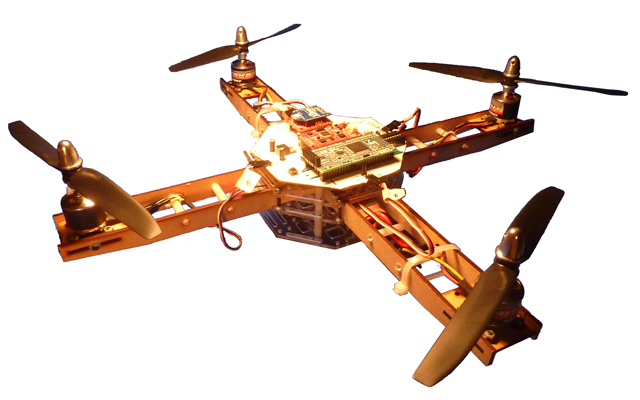
\includegraphics[width=3.25in]{foto_quad.png}
\caption{Prototipo del cuadricóptero}
\label{ref:quadfoto}
\end{figure}

En particular, se trabajó con el objetivo de crear una plataforma abierta y escalable, que le permita a cualquier individuo o grupo empezar a trabajar en el área nutriéndose de los desarrollos presentados y generando un marco para el trabajo en conjunto sobre mejoras y avances. En cuanto al aspecto abierto, se logró utilizando un sistema de documentación tipo wiki, de acceso público, de manera que la información esté disponible universalmente para los individuos o grupos que quieran ponerse a trabajar en la plataforma. El aspecto escalable se logró separando el sistema en subsistemas modulares, de forma que cada subsistema puede ser cambiado y mejorado individualmente sin perjudicar el funcionamiento del conjunto. Se tuvo especial cuidado en la interconexión de la computadora de a bordo con los sensores y en el desarrollo de una arquitectura de capas de abstracción para la computadora de a bordo, que logra la independencia progresiva del software con respecto al hardware. 

La estructura del presente trabajo es la siguiente: primero se describe el diseño y la implementación mecánica y de hardware, luego la arquitectura del software tanto de tierra como de a bordo, luego se resume el estado actual del desarrollo y por último se presenta una breve descripción de las líneas de trabajo que se desprenden del presente trabajo.

\vspace{5 mm}

\section{Diseño Mecánico}

Para el desarrollo del cuadricóptero se comenzó por el diseño de su mecánica estructural. Para que la plataforma sea fácilmente reproducible, se optó por utilizar planchas de corte y una cortadora láser. Esta decisión impactó fuertemente en las posibilidades de diseño, evitando el uso de estructuras tridimensionales y limitando la fabricación a piezas planas. Para la forma del vehículo se propuso una geometría simétrica con dos ejes largos y un octógono central con el fin de colocar la electrónica en el mismo. Con el objetivo de que el proceso de armado del cuadricóptero fuera lo más simple posible, se propuso un sistema de encastre, lo que evita grandes cantidades de elementos de sujeción, reduciendo el peso y a su vez aportando a la simplicidad del diseño. Una foto del prototipo se puede ver en la Fig. \ref{ref:quadfoto}.

\vspace{5 mm}

\section{Arquitectura de Hardware}

Para el diseño de la electrónica de a bordo, se analizaron los requerimientos mínimos para que la plataforma fuera funcional. Como resultado de este análisis, se concluyó que el sistema debería constar de 4 subsistemas principales: 
\begin{itemize}
\item Microcontrolador principal
\item Sensores de navegación 
\item Sistema de comunicación
\item Controlador de velocidad para motores brushless
\end{itemize}
	
El microcontrolador principal elegido fue el LPC1769 de NXP Semiconductors, el cual cuenta con un núcleo ARM Cortex M3.  Este microcontrolador es capaz de ejecutar el algoritmo de control de actitud del vehículo y dispone de un tiempo ocioso estimado en más del 80\%, lo cual permite la implementación de funcionalidades adicionales sin modificar la estructura de a bordo.

Para la elección de los sensores de navegación se consideró que sería interesante que el microcontrolador recibiera información pre-procesada acerca de la actitud del cuadricóptero. Esta elección resultó en la necesidad de utilizar un segundo procesador para el análisis y filtrado de estos sensores. Dados estos requerimientos, se agregó la necesidad de evitar las derivas temporales, ocasionadas por los sensores inerciales relativos, tales como los acelerómetros y giróscopos, los cuales aportan información relativa al cambio de posición y no a la posición absoluta respecto de un eje de referencia dado. Considerando este último requisito y teniendo en cuenta que el cuadricóptero posee un gran espectro de utilidad en recintos cerrados, se descartó el uso de GPS, optando por el uso de magnetómetros, los cuales brindan información acerca de la posición del vehículo respecto al campo magnético del planeta. Finalmente se optó por el desarrollo Razor 9DoF (Degrees of Freedom) IMU (Inertial Measurement Unit) \cite{razor9d0f}, el cual cuenta con sensores de aceleración, giróscopos y magnetómetros alineados para la medición de las magnitudes en una terna ortogonal directa. Esta placa cuenta además con un ATmega328 para el procesamiento de los sensores.

En cuanto a los requerimientos del sistema de comunicación física, se estableció la necesidad de un control de colisiones por parte del hardware, simplificando la programación del microcontrolador principal y liberando tiempo de cálculo para los algoritmos de control y de funcionalidades adicionales. Dado este requisito y estableciendo un rango de utilización de unos pocos cientos de metros, se optó por utilizar los módulos XBee Pro de Digi International, los cuales poseen un control de colisión de paquetes tienen una comunicación sencilla con el microcontrolador, por puerto serie. Esta elección se vio respaldada por la disponibilidad local de los módulos, favoreciendo a la posibilidad de repetición de la plataforma.
Para la elección de los controladores de velocidad de los motores, se optó por la utilización de ESC (Electronic Speed Control) para modelismo. Los mismos son capaces de proporcionar la corriente necesaria para el manejo de los motores y poseen un control del tipo PWM, lo cual aporta a la simplicidad de uso.

Una vez definidos los módulos a utilizar, se diagramó un esquema de interconexión entre los mismos. Dado que el ATmega328 de la placa de sensores se comunica por puerto serie, se designó la conexión del mismo hacia el microcontrolador por ese puerto. Análogamente se fijó la conexión entre el módulo de comunicaciones y el microcontrolador por otro puerto serie. Por último los controladores de velocidad se conectaron a pines del microcontrolador capaces de utilizar PWM por hardware. En la Figura \ref{ref:conexiones} se muestra un esquema de conexionado de las partes.
	
\begin{figure}[btp]
\centering
\includegraphics[width=3.25in]{interconexion.png}
\caption{Esquema de interconexión}
\label{ref:conexiones}
\end{figure}

Considerando los costos de mecánica y de electrónica se estimó un costo de fabricación estimado de 400 dólares.

\vspace{5 mm}

\section{Arquitectura de Software}
Dado que uno de los principales objetivos del proyecto es que éste sea de fácil reproducción y escalabilidad, resulta de vital importancia lograr independencia entre el software y el hardware. Esto permitirá futuras actualizaciones de hardware, con pequeños retoques en el software. Con el fin de lograr este objetivo, se diagramó una estructura de software embebido compuesto por las siguientes partes:
\begin{itemize}
\item HAL (Hardware Abstraction Layer)
\item API  (Application Programming Interface)
\item Aplicación 
\end{itemize}

El HAL es la capa encargada de controlar el hardware, siendo la única específica para el mismo y aportando funciones de manejo de los periféricos de microcontrolador. Esta capa es la única que tendrá acceso directo al hardware y es la única que se deberá modificar ante un eventual cambio del mismo.

La API es la capa que provee al usuario los métodos de programación. Esta capa es intermedia entre el usuario y el HAL. Esta capa no tiene acceso al hardware sino que se ve limitada al uso de las funciones otorgadas por el HAL.

La capa de aplicación es la cual programa el usuario. Esta capa hace uso solamente de la API, no pudiendo acceder directamente al HAL o al hardware. La aplicación será el algoritmo de control, navegación o cualquier otra funcionalidad que el usuario quiera agregar.

Esta división por capas implica una mayor complejidad en la programación de las mismas, pero facilita la portabilidad del código escrito, independizándolo del hardware utilizado, como se mencionó anteriormente. Esta independencia nos permite la migración entre plataformas diferentes, sin la necesidad de reescribir completamente el programa. Esta estructura favorece, además, la escritura del código por parte de terceros, utilizando funciones que elevan el nivel de abstracción de la programación.

En la Figura \ref{ref:soft} se muestra un diagrama de la implementación en las capas previamente descriptas.

\begin{figure}[!t]
\centering
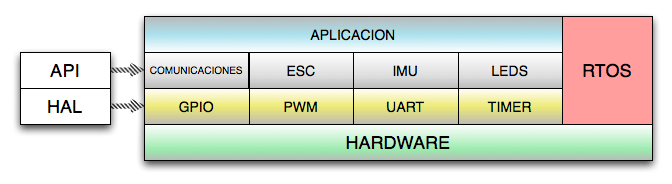
\includegraphics[width=3.49in]{soft}
\caption{Estructura de software}
\label{ref:soft}
\end{figure}

\begin{figure}[!t]
\centering
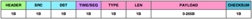
\includegraphics[width=3.40in]{trama}
\caption{Trama del protocolo de comunicaciones}
\label{ref:trama}
\end{figure}

\section{Arquitectura de Comunicaciones}

Para aumentar la confiabilidad y versatilidad del sistema se desarrolló una arquitectura completa para las comunicaciones. Para esto se diseñó un protocolo capaz de detectar errores en las comunicaciones y de transportar paquetes de información entre nodos. Este subsistema se subdividió en cuato capas: Aplicación, Transporte, Enlace, Física.

Las capas físicas y de transporte son íntegramente controladas por los módulos XBee, dejando los modos de direccionamiento a las capas de nivel superior.

La capa de transporte se encarga de que tanto los datos salientes como entrantes cumplan con un determinado formato. Este conformación del paquete permite la detección de errores y la separación de paquetes en función de su utilidad. El módulo de comunicaciones de la capa API de la estructura de software se ocupa de este rol mediante la implementación de una máquina de estados. La comunicación con los módulos XBee la realiza a través del módulo UART de la capa HAL de la estructura de software. 

En la Figura \ref{ref:trama} se muestra el formato de la trama establecida por el protocolo implementado. En la misma se aprecia que la carga útil de la misma es de 0-255Bytes, dejando encargada del fragmentado de los paquetes a la capa de aplicación.
 
 \begin{figure}[!t]
\centering
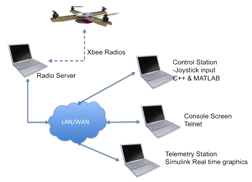
\includegraphics[width=3.45in]{server}
\caption{Esquema de funcionamiento del servidor}
\label{ref:server}
\end{figure}

La capa de transporte es además encargada de verificar la trama mediante las direcciones de fuente y destino, numero de secuencia y checksum. Dado que el protocolo permite interconexión entre diferentes nodos, en ambos sentidos, se requiere un tipo de dato que especifique el carácter de la transmisión (control, telemetría, uplink, downlink). El contenido del payload es presentado a la aplicación de la capa superior que requiere este servicio mediante un modelo publisher/subscriber.

La capa de aplicación implementa la utilidad del protocolo de comunicaciones. Es posible implementar hasta 256 tipos diferentes de datos, diferenciándolos en su propósito. Los tipos de datos implementados actualmente son:
\begin{itemize}
\item System: transmite comandos de sistema, alternando entre modos de funcionamiento del vehículo.
\item Control: transmite información acerca del control de vuelo, tales como cambio en la posición, navegación, acciones, etc.
\item Debug: transmite mensajes de baja prioridad, a interpretarse desde la consola terrestre como caracteres ASCII.
\item Telemetry: transmite paquetes de datos relacionados con la telemetría.
\end{itemize}



\vspace{5 mm}

\section{Implementación del servidor de mensajes}
Como se aprecia en la descripción del protocolo de comunicaciones, el canal estará inundado por diferentes tipos de paquetes, transportando información que será útil a distintos puestos de trabajo. Dado que estos puestos pueden estar ubicados en diferentes locaciones, se implementó un servidor de mensajes, denominado RadioServer. Este servidor se encarga de canalizar las comunicaciones entre los dispositivos de tierra y el cuadricóptero. Ante el arribo de un mensaje, se direccionará el mismo al usuario en cuestión, utilizando puertos TCP. Esta estructura de comunicaciones brinda una gran flexibilidad en cuanto al espectro de utilización del dispositivo, pudiendo desplegar simultáneamente funciones en campo y en laboratorio.
En la Figura \ref{ref:server} se ilustra el funcionamiento del servidor, junto con algunos ejemplos de clientes que se comunican con el cuadricóptero.

\vspace{5 mm}

\section{Trabajo Futuros}

A partir del presente desarrollo queda abierta la posibilidad de comenzar con trabajos sobre temas más puntuales de la ingeniería y operación del cuadricóptero. 

Una línea de trabajo es la mejora mecánica de la plataforma, alivianándola y aumentando la carga útil del cuadricóptero. Esto abre la puerta a nuevas aplicaciones, ya que se pueden transportar más sensores y subsistemas a bordo, como por ejemplo cámaras de fotos, sensores de radiación, nodos de comunicaciones, etc.

Otra línea de trabajo es la mejora de los algoritmos de navegación, lo que le daría más precisión y confiabilidad a la ubicación del cuadricóptero en el espacio y redundaría en más utilidad para los sensores, ya que se contaría con más precisión acerca de dónde fue obtenido el dato. Y también implicaría una mejora en el control del cudricóptero, de la mano de una mejora en los algoritmos de control de actitud y guiado.

Los algoritmos control de actitud y de guiado también son materia de desarrollo actualmente, ya que una mejora en el control de actitud traería asociado más calidad en los datos obtenidos por los sensores, en particular los ópticos como cámaras de fotos, y posibilitaría la autonomía total de la aeronave.

Así mismo se desprende una línea de trabajo consistente en vuelos en formación de más de un cuadricóptero, en la que los controles de las diferentes aeronaves se coordinan entre sí para lograr formaciones estables. Una posible aplicación del vuelo en formación es cubrir un área a sensar con muchos cuadricópteros en un tiempo corto.

Por último, el segmento terreno, es deciri los sistemas en tierra para planificar los vuelos, darle las indicaciones necesarias al cuadricóptero, y procesar los datos recolectados también está abierto a desarrollarse, ya que actualmente solo están implementados los programas necesarios para controlar mínimamente a la aeronave y para mostrar la telemetría recibida.

Actualmente se están desarrollando estas líneas de trabajo tanto en el Laboratorio de Sistemas Embebidos como en el Grupo de Procesamiento de Señales, Identifiación y Control de la Facultad de Ingeniería, Universidad de Buenos Aires.

\vspace{5 mm}

\section*{Conclusión}

Se obtuvo un cuadricóptero totalmente documentado y abierto, que sienta las bases para futuros trabajos de investigación y desarrollo en áreas de control, electrónica y sistemas embebidos. 
Su naturaleza abierta, repetible y escalable lo convierte en una plataforma ideal  para la adaptación relativamente rápida a posibles aplicaciones de sensado y reconocimiento.

\vspace{5 mm}

\section*{Agradecimientos}
Los autores quieren agradecer al Dr. Ing. Juan I. Giribet y al Sr. David Vilaseca por sus valiosos consejos y aportes.

\vspace{5 mm}
% trigger a \newpage just before the given reference
% number - used to balance the columns on the last page
% adjust value as needed - may need to be readjusted if
% the document is modified later
%\IEEEtriggeratref{8}
% The "triggered" command can be changed if desired:
%\IEEEtriggercmd{\enlargethispage{-5in}}

% references section

% can use a bibliography generated by BibTeX as a .bbl file
% BibTeX documentation can be easily obtained at:
% http://www.ctan.org/tex-archive/biblio/bibtex/contrib/doc/
% The IEEEtran BibTeX style support page is at:
% http://www.michaelshell.org/tex/ieeetran/bibtex/
%\bibliographystyle{IEEEtran}
% argument is your BibTeX string definitions and bibliography database(s)
%\bibliography{IEEEabrv,../bib/paper}
\nocite{*}
\bibliographystyle{IEEEtran}
\bibliography{IEEEfull,PresentacionCASE2012}
%
% <OR> manually copy in the resultant .bbl file
% set second argument of \begin to the number of references
% (used to reserve space for the reference number labels box)


%\begin{thebibliography}{1}
%
%\bibitem{IEEEhowto:kopka}
%H.~Kopka and P.~W. Daly, \emph{A Guide to \LaTeX}, 3rd~ed.\hskip 1em plus
%  0.5em minus 0.4em\relax Harlow, England: Addison-Wesley, 1999.
%
%\end{thebibliography}




% that's all folks
\end{document}


